\chapter{Regulator DMC z pomiarem zakłóceń}

\section{Implementacja}

Implementacja regulatora w MatLabie zostanie omówiona za pomocą dobrze udokomunetowanego kodu.

\section {Strojenie regulatora DMC}

Ponieważ środowisko, w którym pracuje regulator nie zmieniło się w stosunku do projektu pierwszego (zerowe zakłócenia Z), dlatego też parametry wtedy otrzymana możne śmiało zastosować i tu. Jednak z uwagi na fakt, iż w ramach poprzedniego projektu strojenie nie odbyło sie w sposób wyczerpujący, teraz sprawdzono kilka innych zestawów parametrów i z nich wybrano najlepszy.\\

\subsection {Badanie parametru $\lambda$}

Poniższe symluacja przeprowadzono dla parametrów N=120 i $N_{u}=20$.\\

\subsubsection{$\lambda$=0,1}

\begin{figure}[h!]
	\centering
	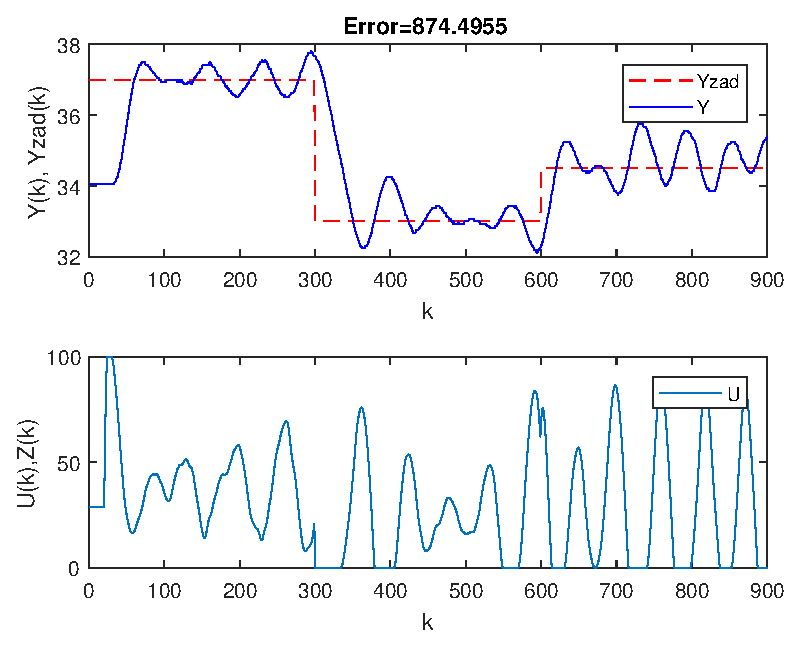
\includegraphics[scale=1]{Rys/N=120Nu=20lambda=0.1.eps}
	\caption{Symulacja regulatora dla $\lambda$=0,1}
	\label{lambda1}
\end{figure}
\FloatBarrier
\subsubsection{$\lambda$=1}

\begin{figure}[h!]
	\centering
	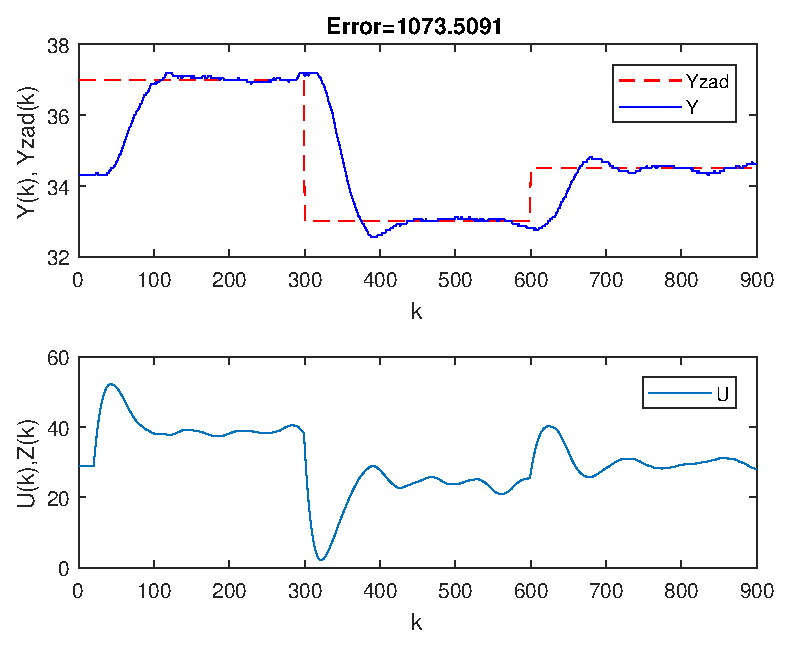
\includegraphics[scale=1]{Rys/N=120Nu=20lambda=1.eps}
	\caption{Symulacja regulatora dla $\lambda$=1}
	\label{lambda2}
\end{figure}
\FloatBarrier
\subsubsection{$\lambda$=10}

\begin{figure}[h!]
	\centering
	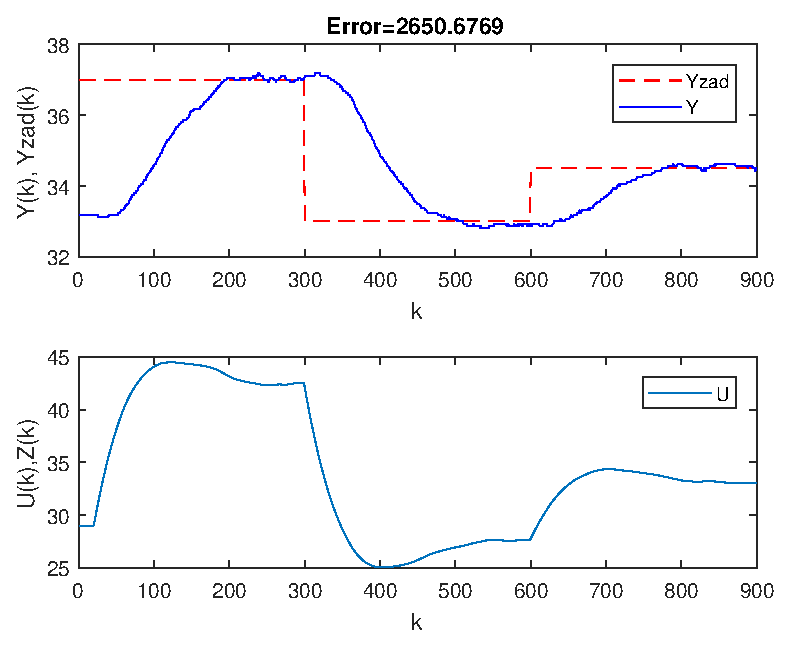
\includegraphics[scale=1]{Rys/N=120Nu=20lambda=10.eps}
	\caption{Symulacja regulatora dla $\lambda$=10}
	\label{lambda3}
\end{figure}

\FloatBarrier

Pod względem błędu (równemu sumie kwadratu odchyłek) regulator dla $\lambda$=0,1, jednak zachowuje się on mniej stabilnie. Regulator dla $\lambda$=1 ma większy błąd, ale wartosci wyjścia i sterowań są mniej zmienne. Wybrano $\lambda$=0,1 do dalszych eksperymentów, gdyż z reguły mniejsze wartosci tego parametru dają lepszą regulację.

\subsection {Badanie parametrów N i $N_{u}$}

\subsubsection{ N=120 $N_{u}$=40}

\begin{figure}[h!]
	\centering
	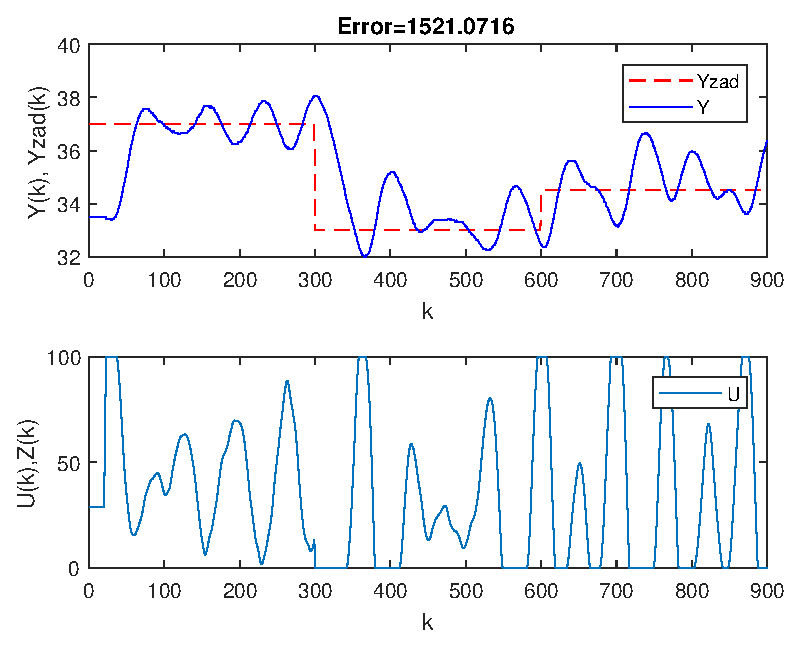
\includegraphics[scale=1]{Rys/N=120Nu=40lambda=0.1.eps}
	\caption{Symulacja regulatora dla N=120 i $N_{u}$=40}
	\label{nnu1}
\end{figure}
\FloatBarrier
\subsubsection{ N=120 $N_{u}$=20}

\begin{figure}[h!]
	\centering
	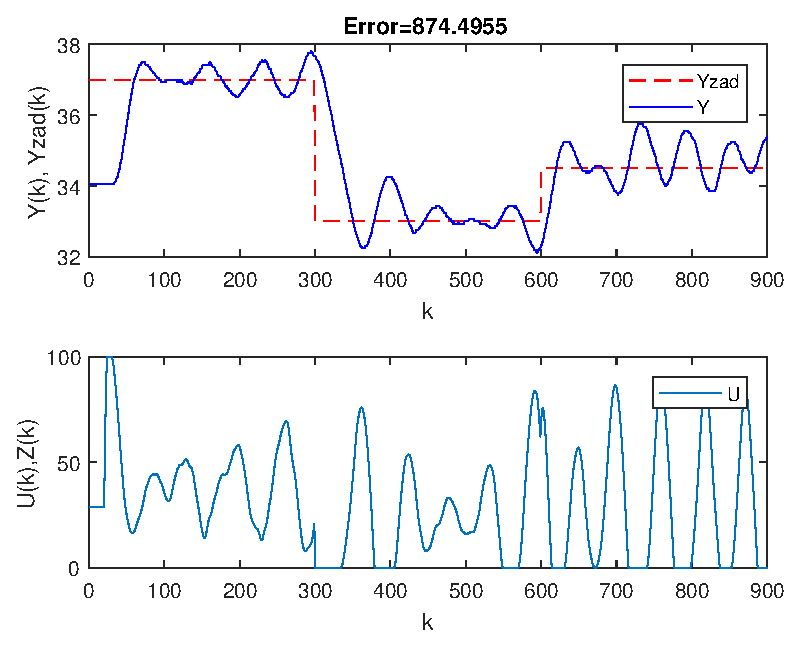
\includegraphics[scale=1]{Rys/N=120Nu=20lambda=0.1.eps}
	\caption{Symulacja regulatora dla N=120 i $N_{u}$=20}
	\label{nnu2}
\end{figure}

\FloatBarrier
\subsubsection{ N=80 $N_{u}$=20}

\begin{figure}[h!]
	\centering
	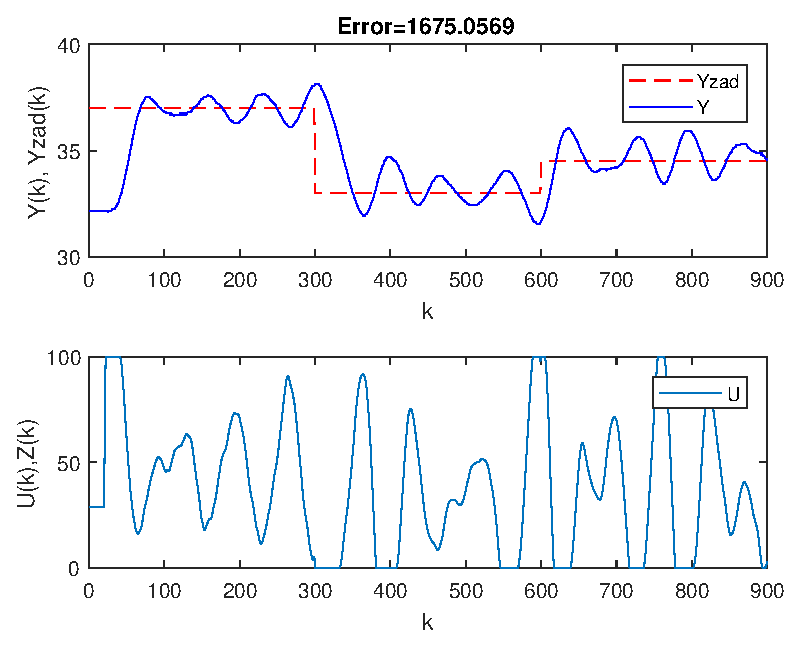
\includegraphics[scale=1]{Rys/N=80Nu=20lambda=0.1.eps}
	\caption{Symulacja regulatora dla N=80 i $N_{u}$=20}
	\label{nnu3}
\end{figure}

\FloatBarrier

Do dalszych eksperymentów wybrano regulator o parametrach   N=120, $N_{u}$=20, $\lambda$=0,1.